\documentclass[a4paper, 12pt]{article}\usepackage[]{graphicx}\usepackage[]{color}
%% maxwidth is the original width if it is less than linewidth
%% otherwise use linewidth (to make sure the graphics do not exceed the margin)
\makeatletter
\def\maxwidth{ %
  \ifdim\Gin@nat@width>\linewidth
    \linewidth
  \else
    \Gin@nat@width
  \fi
}
\makeatother

\definecolor{fgcolor}{rgb}{0.345, 0.345, 0.345}
\newcommand{\hlnum}[1]{\textcolor[rgb]{0.686,0.059,0.569}{#1}}%
\newcommand{\hlstr}[1]{\textcolor[rgb]{0.192,0.494,0.8}{#1}}%
\newcommand{\hlcom}[1]{\textcolor[rgb]{0.678,0.584,0.686}{\textit{#1}}}%
\newcommand{\hlopt}[1]{\textcolor[rgb]{0,0,0}{#1}}%
\newcommand{\hlstd}[1]{\textcolor[rgb]{0.345,0.345,0.345}{#1}}%
\newcommand{\hlkwa}[1]{\textcolor[rgb]{0.161,0.373,0.58}{\textbf{#1}}}%
\newcommand{\hlkwb}[1]{\textcolor[rgb]{0.69,0.353,0.396}{#1}}%
\newcommand{\hlkwc}[1]{\textcolor[rgb]{0.333,0.667,0.333}{#1}}%
\newcommand{\hlkwd}[1]{\textcolor[rgb]{0.737,0.353,0.396}{\textbf{#1}}}%
\let\hlipl\hlkwb

\usepackage{framed}
\makeatletter
\newenvironment{kframe}{%
 \def\at@end@of@kframe{}%
 \ifinner\ifhmode%
  \def\at@end@of@kframe{\end{minipage}}%
  \begin{minipage}{\columnwidth}%
 \fi\fi%
 \def\FrameCommand##1{\hskip\@totalleftmargin \hskip-\fboxsep
 \colorbox{shadecolor}{##1}\hskip-\fboxsep
     % There is no \\@totalrightmargin, so:
     \hskip-\linewidth \hskip-\@totalleftmargin \hskip\columnwidth}%
 \MakeFramed {\advance\hsize-\width
   \@totalleftmargin\z@ \linewidth\hsize
   \@setminipage}}%
 {\par\unskip\endMakeFramed%
 \at@end@of@kframe}
\makeatother

\definecolor{shadecolor}{rgb}{.97, .97, .97}
\definecolor{messagecolor}{rgb}{0, 0, 0}
\definecolor{warningcolor}{rgb}{1, 0, 1}
\definecolor{errorcolor}{rgb}{1, 0, 0}
\newenvironment{knitrout}{}{} % an empty environment to be redefined in TeX

\usepackage{alltt}
\usepackage[utf8]{inputenc}
\usepackage[brazilian, english]{babel}
\usepackage{indentfirst}
\usepackage{graphicx}
\usepackage{float}
\usepackage{titlesec}
\usepackage{amsmath}
\usepackage{caption}
\usepackage{subfigure}
\usepackage{hyperref}
%\usepackage{fixltx2e} %Para subscripts
\usepackage{pgfplots}
\usepackage{textcomp}
\usepackage{enumitem}
\usepackage{multicol}


\title{\textbf{Simulating Exponential Distribution with R in Comparsion with Central Limit Theorem}}
\author{\textit{Eric Calasans de Barros}}
\IfFileExists{upquote.sty}{\usepackage{upquote}}{}
\begin{document}
	\maketitle
	
	\section{Introduction}
	In this project we are make an experiment to verify the central limit theorem(CLT), one of the most important theorems of Statistics, by the simulation of 40 random variables with \textbf{exponential distribution} in a thousand times repeating test.  For each test we take the mean and, at the end, we verify the mean distribution.
	
	\section{Methodology}
		\subsection{Load Packages and Build Data Frame}
		First we load the necessary packages for the task, \textit{dplyr} and \textit{ggplot2}.  Given $\lambda = 0.2$(parameter for exponential distribution) and $n = 40$(number of samples per test), we have the following code:
\begin{knitrout}\small
\definecolor{shadecolor}{rgb}{0.969, 0.969, 0.969}\color{fgcolor}\begin{kframe}
\begin{alltt}
\hlkwd{library}\hlstd{(dplyr)}
\end{alltt}


{\ttfamily\noindent\color{warningcolor}{\#\# Warning: package 'dplyr' was built under R version 3.4.2}}\begin{alltt}
\hlkwd{library}\hlstd{(ggplot2)}

\hlcom{#Parameters for exponential distribution}
\hlstd{lambda} \hlkwb{<-} \hlnum{0.2}
\hlstd{samplesPerTest} \hlkwb{<-} \hlnum{40}
\hlstd{numTests} \hlkwb{<-} \hlnum{1000}

\hlcom{#Matrix of tests}
\hlstd{dataSim} \hlkwb{<-} \hlkwd{rexp}\hlstd{(}\hlkwc{n} \hlstd{= samplesPerTest}\hlopt{*}\hlstd{numTests,lambda)}
\hlstd{testMatrix} \hlkwb{<-} \hlkwd{matrix}\hlstd{(}\hlkwc{data} \hlstd{= dataSim,} \hlkwc{nrow} \hlstd{= numTests)}
\end{alltt}
\end{kframe}
\end{knitrout}
 \subsection{Computation of Sample Mean}
		Now we compute the mean for each line of the matrix as shown below:
\begin{knitrout}\small
\definecolor{shadecolor}{rgb}{0.969, 0.969, 0.969}\color{fgcolor}\begin{kframe}
\begin{alltt}
\hlstd{meanSamples} \hlkwb{<-} \hlkwd{apply}\hlstd{(testMatrix,}\hlnum{1}\hlstd{,mean)}
\hlstd{meanSamplesDF} \hlkwb{<-} \hlkwd{data.frame}\hlstd{(}\hlkwc{means} \hlstd{= meanSamples)}
\end{alltt}
\end{kframe}
\end{knitrout}

        And then, we take the mean of the means in result above:
\begin{knitrout}\small
\definecolor{shadecolor}{rgb}{0.969, 0.969, 0.969}\color{fgcolor}\begin{kframe}
\begin{verbatim}
##  simMean 
## 5.005492
\end{verbatim}
\end{kframe}
\end{knitrout}
        Plotting the histogram, we have:
\begin{knitrout}
\definecolor{shadecolor}{rgb}{0.969, 0.969, 0.969}\color{fgcolor}\begin{kframe}
\begin{alltt}
\hlstd{g}\hlkwb{<-} \hlkwd{ggplot}\hlstd{(meanSamplesDF,}\hlkwd{aes}\hlstd{(}\hlkwc{x} \hlstd{= means) )} \hlopt{+} \hlkwd{geom_histogram}\hlstd{(}\hlkwc{alpha}\hlstd{=}\hlnum{0.4}\hlstd{,}
                        \hlkwc{binwidth}\hlstd{=} \hlnum{.25}\hlstd{,} \hlkwc{fill} \hlstd{=} \hlstr{"blue"}\hlstd{,} \hlkwc{col} \hlstd{=} \hlstr{"black"}\hlstd{)} \hlopt{+}
  \hlkwd{geom_vline}\hlstd{(}\hlkwc{xintercept} \hlstd{= meanSimulation,} \hlkwc{color}\hlstd{=}\hlstr{"red"}\hlstd{,} \hlkwc{size} \hlstd{=} \hlnum{0.5}\hlstd{)} \hlopt{+}
  \hlkwd{ggtitle}\hlstd{(}\hlstr{"Distribution of simulated means"}\hlstd{)}
\hlstd{g}
\end{alltt}
\end{kframe}

{\centering 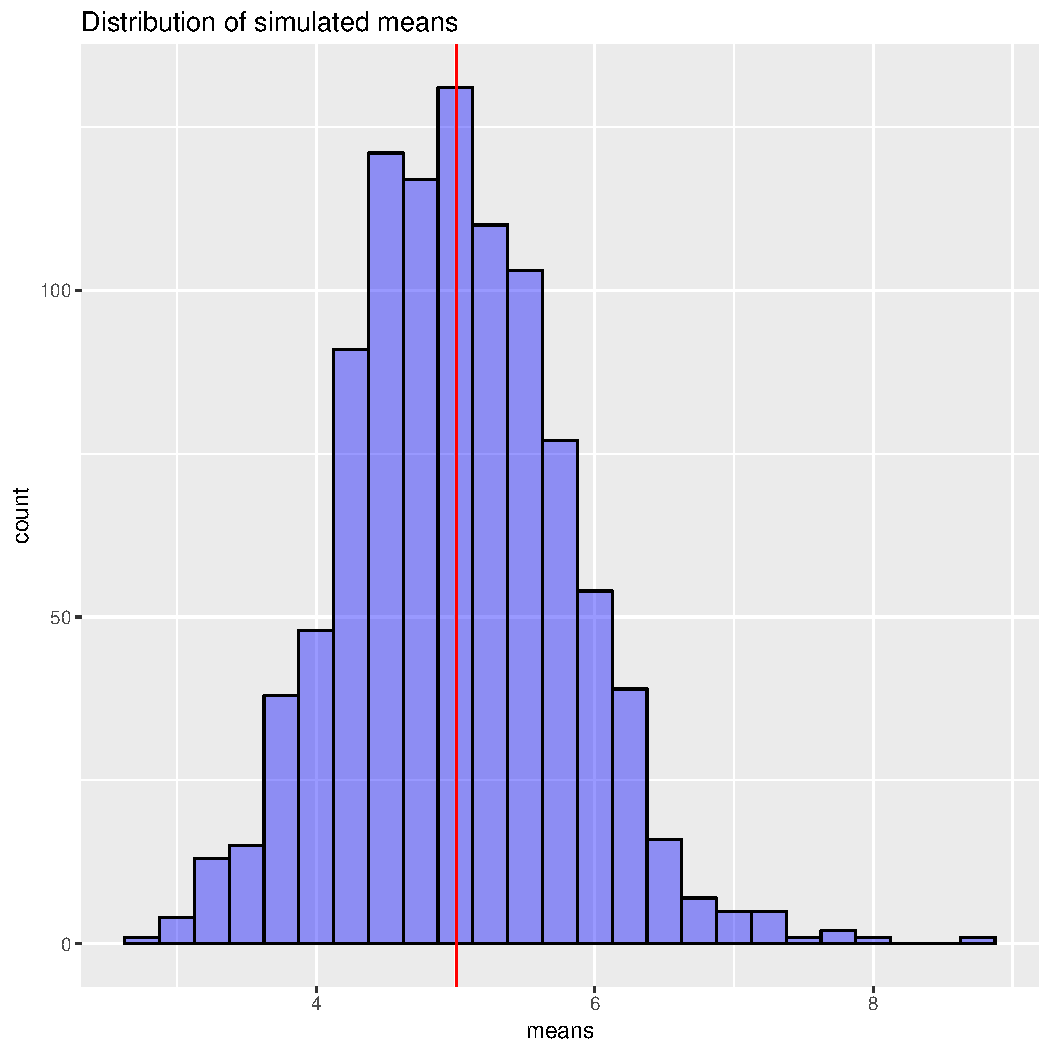
\includegraphics[width=8cm,height=8cm]{figure/plotHistogram-1} 

}



\end{knitrout}
        
	As we can see, the simulated mean, by CLT approaches the theorical mean given by $\frac{1}{\lambda} = 5$.
	
		\subsection{Computation of Sample Variance}
		In this we compute the sample variance in CLT and compare it with the theorical given by $(\frac{\frac{1}{\lambda}}{\sqrt{n}})^2$.
		
\begin{knitrout}\small
\definecolor{shadecolor}{rgb}{0.969, 0.969, 0.969}\color{fgcolor}\begin{kframe}
\begin{alltt}
\hlstd{varSamples} \hlkwb{<-} \hlstd{meanSamplesDF}  \hlopt \hlkwd{select}\hlstd{(means)}  \hlopt \hlkwd{unlist}\hlstd{()} \hlopt  \hlkwd{sd}\hlstd{()}
\hlstd{varSamples} \hlkwb{<-} \hlstd{varSamples} \hlopt{^} \hlnum{2}
\hlstd{varSamples}
\end{alltt}
\begin{verbatim}
## [1] 0.6222146
\end{verbatim}
\end{kframe}
\end{knitrout}

        If $(\frac{\frac{1}{\lambda}}{\sqrt{n}})^2 = 0.625$ we can observe the confirmation of CLT with respect to variance.
        
        \subsection{Normal Distribution}
        	The CLT states that as long as n grows the mean distribution of normalized random variables approaches standard normal distribution(mean = 0 and variance = 1).  That's we intend to show now.  The code below show the procedures:
\begin{knitrout}\small
\definecolor{shadecolor}{rgb}{0.969, 0.969, 0.969}\color{fgcolor}\begin{kframe}
\begin{alltt}
\hlstd{zScore} \hlkwb{<-} \hlstd{(meanSamplesDF}\hlopt{$}\hlstd{means} \hlopt{-} \hlstd{(}\hlnum{1}\hlopt{/}\hlstd{lambda))}
\hlstd{zScore} \hlkwb{<-} \hlstd{zScore}\hlopt{/}\hlstd{(}\hlnum{1}\hlopt{/}\hlstd{lambda}\hlopt{/}\hlkwd{sqrt}\hlstd{(samplesPerTest))}
\hlstd{zMean} \hlkwb{<-} \hlkwd{mean}\hlstd{(zScore)}
\hlstd{zMean}
\end{alltt}
\begin{verbatim}
## [1] 0.006947234
\end{verbatim}
\end{kframe}
\end{knitrout}
        Then we plot:
\begin{knitrout}
\definecolor{shadecolor}{rgb}{0.969, 0.969, 0.969}\color{fgcolor}\begin{kframe}
\begin{alltt}
\hlstd{zPlot} \hlkwb{<-} \hlkwd{ggplot}\hlstd{(}\hlkwd{as.data.frame}\hlstd{(zScore),} \hlkwd{aes}\hlstd{(}\hlkwc{x} \hlstd{= zScore))} \hlopt{+}
   \hlkwd{geom_histogram}\hlstd{(}\hlkwc{alpha}\hlstd{=}\hlnum{0.1}\hlstd{,}  \hlkwc{binwidth} \hlstd{=} \hlnum{0.3}\hlstd{,} \hlkwc{fill}\hlstd{=}\hlstr{"yellow"}\hlstd{,}
                  \hlkwc{color}\hlstd{=}\hlstr{"black"}\hlstd{,} \hlkwd{aes}\hlstd{(}\hlkwc{y} \hlstd{= ..density..))} \hlopt{+}
   \hlkwd{stat_function}\hlstd{(}\hlkwc{fun} \hlstd{= dnorm,} \hlkwc{size} \hlstd{=} \hlnum{1.3}\hlstd{)} \hlopt{+}
   \hlkwd{geom_vline}\hlstd{(}\hlkwc{xintercept} \hlstd{= zMean,} \hlkwc{color}\hlstd{=}\hlstr{"red"}\hlstd{,} \hlkwc{size} \hlstd{=} \hlnum{0.5}\hlstd{)} \hlopt{+}
   \hlkwd{ggtitle}\hlstd{(}\hlstr{"Distribution of standardized \textbackslash{}nsimulated means"}\hlstd{)} \hlopt{+}
   \hlkwd{xlab}\hlstd{(}\hlstr{"z-scores"}\hlstd{)}
\hlstd{zPlot}
\end{alltt}
\end{kframe}

{\centering 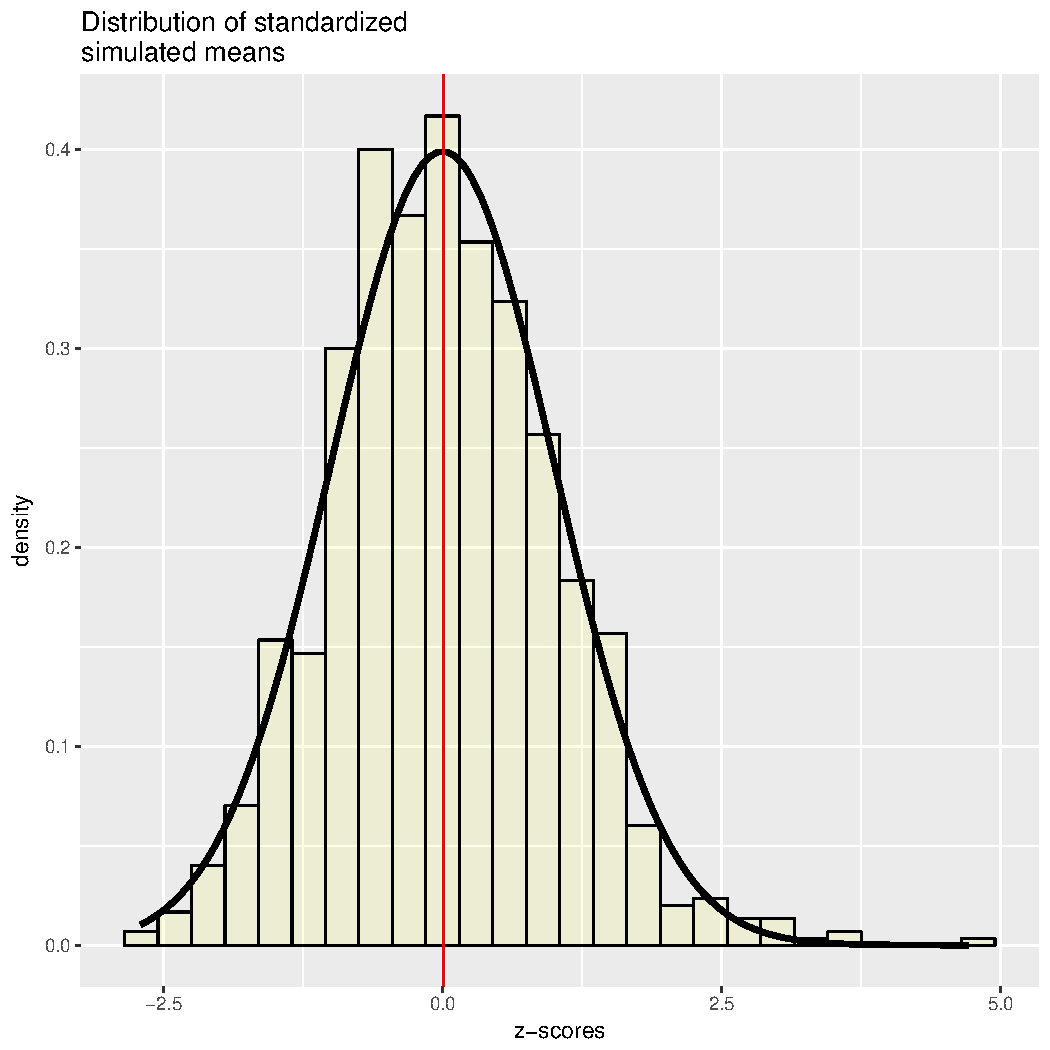
\includegraphics[width=8cm,height=8cm]{figure/plotZ-1} 

}



\end{knitrout}
        
\end{document}


